%% This style is provided for the ICSE 2015 main conference,
%% ICSE 2015 co-located events, and ICSE 2015 workshops.

%% bare_conf_ICSE15.tex
%% V1.4
%% 2014/05/22


%% This is a skeleton file demonstrating the use of IEEEtran.cls
%% (requires IEEEtran.cls version 1.7 or later) with an IEEE conference paper.
%%
%% Support sites:
%% http://www.michaelshell.org/tex/ieeetran/
%% http://www.ctan.org/tex-archive/macros/latex/contrib/IEEEtran/
%% and
%% http://www.ieee.org/

%%*************************************************************************
%% Legal Notice:
%% This code is offered as-is without any warranty either expressed or
%% implied; without even the implied warranty of MERCHANTABILITY or
%% FITNESS FOR A PARTICULAR PURPOSE!
%% User assumes all risk.
%% In no event shall IEEE or any contributor to this code be liable for
%% any damages or losses, including, but not limited to, incidental,
%% consequential, or any other damages, resulting from the use or misuse
%% of any information contained here.
%%
%% All comments are the opinions of their respective authors and are not
%% necessarily endorsed by the IEEE.
%%
%% This work is distributed under the LaTeX Project Public License (LPPL)
%% ( http://www.latex-project.org/ ) version 1.3, and may be freely used,
%% distributed and modified. A copy of the LPPL, version 1.3, is included
%% in the base LaTeX documentation of all distributions of LaTeX released
%% 2003/12/01 or later.
%% Retain all contribution notices and credits.
%% ** Modified files should be clearly indicated as such, including  **
%% ** renaming them and changing author support contact information. **
%%
%% File list of work: IEEEtran.cls, IEEEtran_HOWTO.pdf, bare_adv.tex,
%%                    bare_conf.tex, bare_jrnl.tex, bare_jrnl_compsoc.tex
%%*************************************************************************

% *** Authors should verify (and, if needed, correct) their LaTeX system  ***
% *** with the testflow diagnostic prior to trusting their LaTeX platform ***
% *** with production work. IEEE's font choices can trigger bugs that do  ***
% *** not appear when using other class files.                            ***
% The testflow support page is at:
% http://www.michaelshell.org/tex/testflow/



% Note that the a4paper option is mainly intended so that authors in
% countries using A4 can easily print to A4 and see how their papers will
% look in print - the typesetting of the document will not typically be
% affected with changes in paper size (but the bottom and side margins will).
% Use the testflow package mentioned above to verify correct handling of
% both paper sizes by the user's LaTeX system.
%
% Also note that the "draftcls" or "draftclsnofoot", not "draft", option
% should be used if it is desired that the figures are to be displayed in
% draft mode.
%
\documentclass[conference]{IEEEtran}
%
% If IEEEtran.cls has not been installed into the LaTeX system files,
% manually specify the path to it like:
% \documentclass[conference]{../sty/IEEEtran}





% Some very useful LaTeX packages include:
% (uncomment the ones you want to load)


% *** MISC UTILITY PACKAGES ***
%
%\usepackage{ifpdf}
% Heiko Oberdiek's ifpdf.sty is very useful if you need conditional
% compilation based on whether the output is pdf or dvi.
% usage:
% \ifpdf
%   % pdf code
% \else
%   % dvi code
% \fi
% The latest version of ifpdf.sty can be obtained from:
% http://www.ctan.org/tex-archive/macros/latex/contrib/oberdiek/
% Also, note that IEEEtran.cls V1.7 and later provides a builtin
% \ifCLASSINFOpdf conditional that works the same way.
% When switching from latex to pdflatex and vice-versa, the compiler may
% have to be run twice to clear warning/error messages.






% *** CITATION PACKAGES ***
%
\usepackage{cite}
% cite.sty was written by Donald Arseneau
% V1.6 and later of IEEEtran pre-defines the format of the cite.sty package
% \cite{} output to follow that of IEEE. Loading the cite package will
% result in citation numbers being automatically sorted and properly
% "compressed/ranged". e.g., [1], [9], [2], [7], [5], [6] without using
% cite.sty will become [1], [2], [5]--[7], [9] using cite.sty. cite.sty's
% \cite will automatically add leading space, if needed. Use cite.sty's
% noadjust option (cite.sty V3.8 and later) if you want to turn this off.
% cite.sty is already installed on most LaTeX systems. Be sure and use
% version 4.0 (2003-05-27) and later if using hyperref.sty. cite.sty does
% not currently provide for hyperlinked citations.
% The latest version can be obtained at:
% http://www.ctan.org/tex-archive/macros/latex/contrib/cite/
% The documentation is contained in the cite.sty file itself.






% *** GRAPHICS RELATED PACKAGES ***
%
\ifCLASSINFOpdf
  \usepackage[pdftex]{graphicx}
  \usepackage{subfig}
  % declare the path(s) where your graphic files are
  % \graphicspath{{../pdf/}{../jpeg/}}
  % and their extensions so you won't have to specify these with
  % every instance of \includegraphics
  \DeclareGraphicsExtensions{.pdf,.jpeg,.png}
\else
  % or other class option (dvipsone, dvipdf, if not using dvips). graphicx
  % will default to the driver specified in the system graphics.cfg if no
  % driver is specified.
  % \usepackage[dvips]{graphicx}
  % declare the path(s) where your graphic files are
  % \graphicspath{{../eps/}}
  % and their extensions so you won't have to specify these with
  % every instance of \includegraphics
  % \DeclareGraphicsExtensions{.eps}
\fi
% graphicx was written by David Carlisle and Sebastian Rahtz. It is
% required if you want graphics, photos, etc. graphicx.sty is already
% installed on most LaTeX systems. The latest version and documentation can
% be obtained at:
% http://www.ctan.org/tex-archive/macros/latex/required/graphics/
% Another good source of documentation is "Using Imported Graphics in
% LaTeX2e" by Keith Reckdahl which can be found as epslatex.ps or
% epslatex.pdf at: http://www.ctan.org/tex-archive/info/
%
% latex, and pdflatex in dvi mode, support graphics in encapsulated
% postscript (.eps) format. pdflatex in pdf mode supports graphics
% in .pdf, .jpeg, .png and .mps (metapost) formats. Users should ensure
% that all non-photo figures use a vector format (.eps, .pdf, .mps) and
% not a bitmapped formats (.jpeg, .png). IEEE frowns on bitmapped formats
% which can result in "jaggedy"/blurry rendering of lines and letters as
% well as large increases in file sizes.
%
% You can find documentation about the pdfTeX application at:
% http://www.tug.org/applications/pdftex





% *** MATH PACKAGES ***
%
%\usepackage[cmex10]{amsmath}
% A popular package from the American Mathematical Society that provides
% many useful and powerful commands for dealing with mathematics. If using
% it, be sure to load this package with the cmex10 option to ensure that
% only type 1 fonts will utilized at all point sizes. Without this option,
% it is possible that some math symbols, particularly those within
% footnotes, will be rendered in bitmap form which will result in a
% document that can not be IEEE Xplore compliant!
%
% Also, note that the amsmath package sets \interdisplaylinepenalty to 10000
% thus preventing page breaks from occurring within multiline equations. Use:
%\interdisplaylinepenalty=2500
% after loading amsmath to restore such page breaks as IEEEtran.cls normally
% does. amsmath.sty is already installed on most LaTeX systems. The latest
% version and documentation can be obtained at:
% http://www.ctan.org/tex-archive/macros/latex/required/amslatex/math/





% *** SPECIALIZED LIST PACKAGES ***
%
%\usepackage{algorithmic}
% algorithmic.sty was written by Peter Williams and Rogerio Brito.
% This package provides an algorithmic environment fo describing algorithms.
% You can use the algorithmic environment in-text or within a figure
% environment to provide for a floating algorithm. Do NOT use the algorithm
% floating environment provided by algorithm.sty (by the same authors) or
% algorithm2e.sty (by Christophe Fiorio) as IEEE does not use dedicated
% algorithm float types and packages that provide these will not provide
% correct IEEE style captions. The latest version and documentation of
% algorithmic.sty can be obtained at:
% http://www.ctan.org/tex-archive/macros/latex/contrib/algorithms/
% There is also a support site at:
% http://algorithms.berlios.de/index.html
% Also of interest may be the (relatively newer and more customizable)
% algorithmicx.sty package by Szasz Janos:
% http://www.ctan.org/tex-archive/macros/latex/contrib/algorithmicx/




% *** ALIGNMENT PACKAGES ***
%
%\usepackage{array}
% Frank Mittelbach's and David Carlisle's array.sty patches and improves
% the standard LaTeX2e array and tabular environments to provide better
% appearance and additional user controls. As the default LaTeX2e table
% generation code is lacking to the point of almost being broken with
% respect to the quality of the end results, all users are strongly
% advised to use an enhanced (at the very least that provided by array.sty)
% set of table tools. array.sty is already installed on most systems. The
% latest version and documentation can be obtained at:
% http://www.ctan.org/tex-archive/macros/latex/required/tools/


%\usepackage{mdwmath}
%\usepackage{mdwtab}
% Also highly recommended is Mark Wooding's extremely powerful MDW tools,
% especially mdwmath.sty and mdwtab.sty which are used to format equations
% and tables, respectively. The MDWtools set is already installed on most
% LaTeX systems. The lastest version and documentation is available at:
% http://www.ctan.org/tex-archive/macros/latex/contrib/mdwtools/


% IEEEtran contains the IEEEeqnarray family of commands that can be used to
% generate multiline equations as well as matrices, tables, etc., of high
% quality.


%\usepackage{eqparbox}
% Also of notable interest is Scott Pakin's eqparbox package for creating
% (automatically sized) equal width boxes - aka "natural width parboxes".
% Available at:
% http://www.ctan.org/tex-archive/macros/latex/contrib/eqparbox/





% *** SUBFIGURE PACKAGES ***
%\usepackage[tight,footnotesize]{subfigure}
% subfigure.sty was written by Steven Douglas Cochran. This package makes it
% easy to put subfigures in your figures. e.g., "Figure 1a and 1b". For IEEE
% work, it is a good idea to load it with the tight package option to reduce
% the amount of white space around the subfigures. subfigure.sty is already
% installed on most LaTeX systems. The latest version and documentation can
% be obtained at:
% http://www.ctan.org/tex-archive/obsolete/macros/latex/contrib/subfigure/
% subfigure.sty has been superceeded by subfig.sty.



%\usepackage[caption=false]{caption}
%\usepackage[font=footnotesize]{subfig}
% subfig.sty, also written by Steven Douglas Cochran, is the modern
% replacement for subfigure.sty. However, subfig.sty requires and
% automatically loads Axel Sommerfeldt's caption.sty which will override
% IEEEtran.cls handling of captions and this will result in nonIEEE style
% figure/table captions. To prevent this problem, be sure and preload
% caption.sty with its "caption=false" package option. This is will preserve
% IEEEtran.cls handing of captions. Version 1.3 (2005/06/28) and later
% (recommended due to many improvements over 1.2) of subfig.sty supports
% the caption=false option directly:
%\usepackage[caption=false,font=footnotesize]{subfig}
%
% The latest version and documentation can be obtained at:
% http://www.ctan.org/tex-archive/macros/latex/contrib/subfig/
% The latest version and documentation of caption.sty can be obtained at:
% http://www.ctan.org/tex-archive/macros/latex/contrib/caption/




% *** FLOAT PACKAGES ***
%
%\usepackage{fixltx2e}
% fixltx2e, the successor to the earlier fix2col.sty, was written by
% Frank Mittelbach and David Carlisle. This package corrects a few problems
% in the LaTeX2e kernel, the most notable of which is that in current
% LaTeX2e releases, the ordering of single and double column floats is not
% guaranteed to be preserved. Thus, an unpatched LaTeX2e can allow a
% single column figure to be placed prior to an earlier double column
% figure. The latest version and documentation can be found at:
% http://www.ctan.org/tex-archive/macros/latex/base/



%\usepackage{stfloats}
% stfloats.sty was written by Sigitas Tolusis. This package gives LaTeX2e
% the ability to do double column floats at the bottom of the page as well
% as the top. (e.g., "\begin{figure*}[!b]" is not normally possible in
% LaTeX2e). It also provides a command:
%\fnbelowfloat
% to enable the placement of footnotes below bottom floats (the standard
% LaTeX2e kernel puts them above bottom floats). This is an invasive package
% which rewrites many portions of the LaTeX2e float routines. It may not work
% with other packages that modify the LaTeX2e float routines. The latest
% version and documentation can be obtained at:
% http://www.ctan.org/tex-archive/macros/latex/contrib/sttools/
% Documentation is contained in the stfloats.sty comments as well as in the
% presfull.pdf file. Do not use the stfloats baselinefloat ability as IEEE
% does not allow \baselineskip to stretch. Authors submitting work to the
% IEEE should note that IEEE rarely uses double column equations and
% that authors should try to avoid such use. Do not be tempted to use the
% cuted.sty or midfloat.sty packages (also by Sigitas Tolusis) as IEEE does
% not format its papers in such ways.





% *** PDF, URL AND HYPERLINK PACKAGES ***
%
\usepackage{url}
% url.sty was written by Donald Arseneau. It provides better support for
% handling and breaking URLs. url.sty is already installed on most LaTeX
% systems. The latest version can be obtained at:
% http://www.ctan.org/tex-archive/macros/latex/contrib/misc/
% Read the url.sty source comments for usage information. Basically,
% \url{my_url_here}.





% *** Do not adjust lengths that control margins, column widths, etc. ***
% *** Do not use packages that alter fonts (such as pslatex).         ***
% There should be no need to do such things with IEEEtran.cls V1.6 and later.
% (Unless specifically asked to do so by the journal or conference you plan
% to submit to, of course. )


% correct bad hyphenation here
\hyphenation{op-tical net-works semi-conduc-tor}


\begin{document}
%
% paper title
% can use linebreaks \\ within to get better formatting as desired
\title{Continuous Deployment and Schema Evolution \\in SQL Databases}


% author names and affiliations
% use a multiple column layout for up to three different
% affiliations
%\author{\IEEEauthorblockN{Michael Shell}
%\IEEEauthorblockA{School of Electrical and\\Computer Engineering\\
%Georgia Institute of Technology\\
%Atlanta, Georgia 30332--0250\\
%Email: http://www.michaelshell.org/contact.html}
%\and
%\IEEEauthorblockN{Homer Simpson}
%\IEEEauthorblockA{Twentieth Century Fox\\
%Springfield, USA\\
%Email: homer@thesimpsons.com}
%\and
%\IEEEauthorblockN{James Kirk\\ and Montgomery Scott}
%\IEEEauthorblockA{Starfleet Academy\\
%San Francisco, California 96678-2391\\
%Telephone: (800) 555--1212\\
%Fax: (888) 555--1212}}

% conference papers do not typically use \thanks and this command
% is locked out in conference mode. If really needed, such as for
% the acknowledgment of grants, issue a \IEEEoverridecommandlockouts
% after \documentclass

% for over three affiliations, or if they all won't fit within the width
% of the page, use this alternative format:
%



\author{
  \IEEEauthorblockN{
    Michael de Jong\IEEEauthorrefmark{1},
    Arie van Deursen\IEEEauthorrefmark{2}
  }
  \IEEEauthorblockA{
    Delft University of Technology,\\
    Delft, The Netherlands\\ \\
    Email: M.deJong-2@student.tudelft.nl\IEEEauthorrefmark{1}\\
    Email: Arie.vanDeursen@tudelft.nl\IEEEauthorrefmark{2}\\ \\
    \today{}
  }
}



% use for special paper notices
%\IEEEspecialpapernotice{(Invited Paper)}




% make the title area
\maketitle


\begin{abstract}
%\boldmath

Continuous Deployment is an important enabler of rapid delivery of business value and early end user feedback. While frequent code deployment is well understood, the impact of frequent change on persistent data is less understood and supported. SQL schema evolutions in particular can make it expensive to deploy a new version, and may even lead to downtime if schema changes can only be applied by blocking operations.

In this paper we study the problem of continuous deployment in the presence of database schema evolution in more detail. We identify a number of shortcomings to existing solutions and tools, mostly related to avoidable downtime and support for foreign keys. We propose a novel approach to address these problems, and provide an open source implementation. Initial evaluation suggests the approach is effective and sufficiently efficient.


\end{abstract}
% IEEEtran.cls defaults to using nonbold math in the Abstract.
% This preserves the distinction between vectors and scalars. However,
% if the conference you are submitting to favors bold math in the abstract,
% then you can use LaTeX's standard command \boldmath at the very start
% of the abstract to achieve this. Many IEEE journals/conferences frown on
% math in the abstract anyway.

% no keywords




% For peer review papers, you can put extra information on the cover
% page as needed:
% \ifCLASSOPTIONpeerreview
% \begin{center} \bfseries EDICS Category: 3-BBND \end{center}
% \fi
%
% For peerreview papers, this IEEEtran command inserts a page break and
% creates the second title. It will be ignored for other modes.
\IEEEpeerreviewmaketitle



\section{Introduction} %(0.7)

% * Problem from RelEng viewpoint.
% * Blocking nature of DDL statements.
% * Continuous Deployment and partial deployments.

SQL databases are an integral part of many (web) applications. They provide strong guarantees about the storage and retrieval of persistent data which makes them useful for various software applications. 

For release engineers, the persistence of the data and especially the structure of this data as embedded in the application's SQL schema is at odds with today's need for continuous deployment. Challenges include combining zero downtime constraints with evolving database schemas (affecting tables, columns, foreign keys, constraints, etc.), and the need to be able to rollback changes without loss of data.

We can distill the challenge of continuous delivery in the presence of schema evolution into two separate problems:

First, given the deployment of a new version of a (web) application, depending on the deployment strategy it might be required that both the old and the new version of the application run in parallel (\textit{Rolling Upgrades}, or \textit{Canary Releases}~\cite{Humble:2010:CDR:1869904}). This means that the schema on the SQL database needs to be compatible with the schema expected by both the old and the new version of the application.

Second, operations which modify the database schema in a SQL database (\textit{DDL statements}) can be either non-blocking or blocking in nature, depending on the implementation of the operations in that specific SQL database. In case of non-blocking \textit{DDL statements}, SQL queries issued by the application may proceed, whereas with blocking \textit{DDL statements} these queries may be put on hold for the duration of the operation. This disruption can range from milliseconds to hours depending on the schema operation, the size of the affected table(s), and the database implementation. One such example would be adding a new non-nullable column to an existing table in a PostgreSQL database. This operation is blocking in nature, preventing other queries from running while it is being executed. When applied to a table of 50 million records (see Section~\ref{sec:results}), the queries from the application can be blocked for 2.5 minutes.


When service windows are short or even non-existent, these two problems make releasing new versions of applications frequently problematic for release engineers. To address this problem we aim to find or implement a tool which allows its users to not only alter their database schema in a non-blocking fashion, but also do this without affecting older applications still operating on the older version of the schema.

\section{State of the Art} %(0.7)

% * Manual approach
% * Automated tools in academia and industry
% * Limitations of approaches

\subsection{Continuous Delivery}\label{sec:cd}

We first examine existing approaches, tools, and research aiming to solve these problems. Our starting point is the seminal book ``Continuous Delivery''~\cite{Humble:2010:CDR:1869904}. This book describes three high-level approaches to deal with migrating data without loss of data or requiring downtime:

\begin{itemize}
  \item{\textbf{Approach 1}: Copy the database or schema and start recording transactions. When the copying has completed, apply the schema changes to the copied database or schema. Finally replay all the recorded database transactions on the copied database or schema to reach an equivalent state. Once this state has been achieved, it must either be maintained by continuing to record and playback transactions, or make the switch from the old to the new database or schema.}
  \item{\textbf{Approach 2}: When using \textit{Blue-Green deployments}, two instances of the database are available. Take the inactive database and apply the schema operations to it. In the mean time these two databases need to be kept synchronized. This can be done by using approach 1, or somehow ensure that the table under change remains in a read-only state until the active and inactive databases have switched roles.}
  \item{\textbf{Approach 3}: The last is an approach where schema operations are performed separately from the application deployments using operations which are non-blocking. As a consequence the application must be able to deal with either the old or the new database schema being in use, and construct SQL queries which can operate correctly on both schemas.}
\end{itemize}

\subsection{Current Tooling} 
Since evolving the schema of a database and coordinating the deployment of software are both complex tasks, we looked for tooling which could help automate this for software and release engineers.

\subsubsection{Percona Toolkit~\cite{PerconaToolkit} \& Openark Kit~\cite{OpenarkKit}}
These are tools designed to help DBAs perform administrative tasks on MySQL databases. The commands \textit{oak-online-alter-table} and \textit{pt-online-schema-change} create an empty copy of the a specified table (a ghost table) and apply schema operations to the ghost table. These commands then proceed to install triggers on both tables, which insert, update, or delete the corresponding record in the other table when a record in their own table is inserted, updated, or deleted. A background task iterates over all records in the original table (in batches) and lazily copies records from the original table to the ghost table. When all records have been copied the original table and ghost table switch names atomically, ensuring that clients now use the ghost table when querying the original table name.

\subsubsection{TableMigrator~\cite{TableMigrator}}
This is a tool which works like Openark Kit and Percona Toolkit. Instead of using triggers to synchronize the two tables with each other,  TableMigrator requires tables to have an additional column which stores the date and time that record was last modified. Using this information corresponding records in both tables are synchronized with each other by passing over all records in multiple passes. Once a pass can be done relatively quickly, TableMigrator acquires an exclusive write lock on the original table --- blocking the entire table --- and proceeds to do a final pass. Once this has been done, it atomically swaps the names of the original and ghost table before releasing the write lock. Since this final pass can be done quickly, any application executing queries on that table is only very briefly blocked.

\subsubsection{SoundCloud's Large Hadron Migrator~\cite{SoundcloudLHM} \& Facebook's Online Schema Change~\cite{FacebookOSC}}
These are both tools which closely follow Approach~1 described earlier (Section~\ref{sec:cd}). They create a copy of a table (including its contents) and record modifications to records in the original table using triggers into a special ``deltas'' table. Once they have copied the original table and its contents, they apply the specified schema operations to the ghost table before proceeding to replay the recorded modifications from the ``deltas'' table onto the ghost table. When the ``deltas'' table is almost empty, these tools acquire an exclusive write lock on the original table --- like \textit{TableMigrator} does --- and apply the last of the recorded modifications before atomically switch the names of both tables.

\subsection{Research}

\subsubsection{Imago}
Imago~\cite{Dumitras:2009:WUF:1656980.1657005} is a tool which follows Approach~2. With Imago there are two production environments, called ``universes''. Imago integrates with the application and its environment at both the ingress point (load balancer) to be able to switch users from one ``universe'' to the other, and at the egress point where the (web) application sends queries to the SQL database. When a new version of the application (requiring a change to the database schema) needs to be deployed, Imago bootstraps the inactive production environment with a copy of the active database, applies the required schema operations and then copies over the data from the old universe to the new universe. When this process is almost complete, it enforces a short period of read-only access to the SQL database, while it is switching users from the old ``universe'' to the new ``universe'' using the load balancer. Imago makes no claims in regards to its support for foreign keys.

\subsection{Limitations} 

\begin{itemize}
  \item None of the tools used in practice support foreign keys.
  \item The tools primarily focus on MySQL databases.
  \item These tools are limited in the sense that they typically only support making small changes to the existing database schema. This forces software and release engineers to often release intermediate versions of the application, as the schema is altered in several steps.
\end{itemize}

\section{Proposed Approach} %(1.0)

\subsection{Vision}

We feel that the current situation is an impediment to the adoption of \textit{Continuous Deployment}. Although \textit{Continuous Deployment} has made great improvements on workflows, team dynamics, and tooling for deploying and monitoring applications, the area of schema evolution in databases has received little attention. Therefore we aim to address these problems by developing a new tool which adheres to the following principles:

\begin{itemize}
  \item{A solution should not put restrictions on how to deploy applications, or which methods of deployment can be used: \textit{Blue-Green deployments}, \textit{Rolling upgrades}, \textit{Canary releases}, etc.}
  \item{Clients connected to the database must be able to access the contents of the database according to an active version of the database schema of their choosing. Their ``view'' should only contain tables, columns, foreign keys, etc which are present in their chosen version of the database schema, but contain the same data as is present in all other ``views''.}
  \item{Versioning and rolling back are important for release engineers. A solution should support versioning the changes being made to the database schema, and be able to rollback to a previous version if the need arises.}
  \item{Foreign keys are an integral part of SQL databases and should be supported.}
\end{itemize}

\subsection{Solution Direction}

The previously discussed tools from practice all use Approach~1 or a variation of it. They prove that this is a viable way for simple evolutions of the database schema. However where these tools all create a single ghost table, we aim to create one ghost table for each table that is under change, and ghost tables for all tables which in turn are dependent on these tables under change. For instance adding a new non-nullable column ``summary'' to the ``books'' table (see Figure~\ref{fig:migration-stages}), means we should also create a ghost table for the ``publications`` table since there is a foreign key pointing from the ``publications'' table to the ``books'' table. The other tables do not require ghost tables, as they do not have any foreign keys referencing either the ``books'' or ``publications'' table. This approach ensures that we can support foreign keys.

In addition, the tools from practice all allow release engineers to switch the table names manually after the the original and the ghost table have been synchronized. This allows for two or more versions of the application to co-exist on the same database as long as each version correctly queries the correct (ghost) table. Although the current tools from practice do not solve this specific problem, we think that this is easily solved using a small wrapper around database drivers for most programming languages.

Finally, with this approach it is possible to perform several schema evolutions at once. In the example, we could for instance also add even more columns to either the ``books'' or ``publications'' table.

\section{Implementation Status} %(0.5)

\subsection{Current Status}

We are in the process of implementing and experimenting with the approach just described via a new tool that we have named QuantumDB~\cite{QuantumDB}.
The aim is to make \textit{Continuous Deployment} more attainable for software and release engineers for applications relying on SQL databases. Although not yet ready for production environments, we have implemented enough to perform a quick evaluation in a small experiment. 

\begin{figure}%
    \centering
    \subfloat[Original database schema, before migration]{{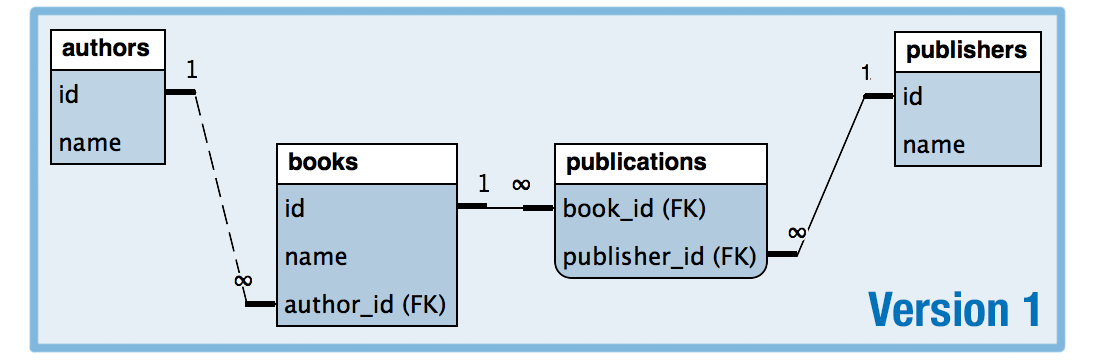
\includegraphics[width=3.0in]{pre-migration-state.png} }}%
    \qquad
    \subfloat[Database schema in mixed-state, during migration]{{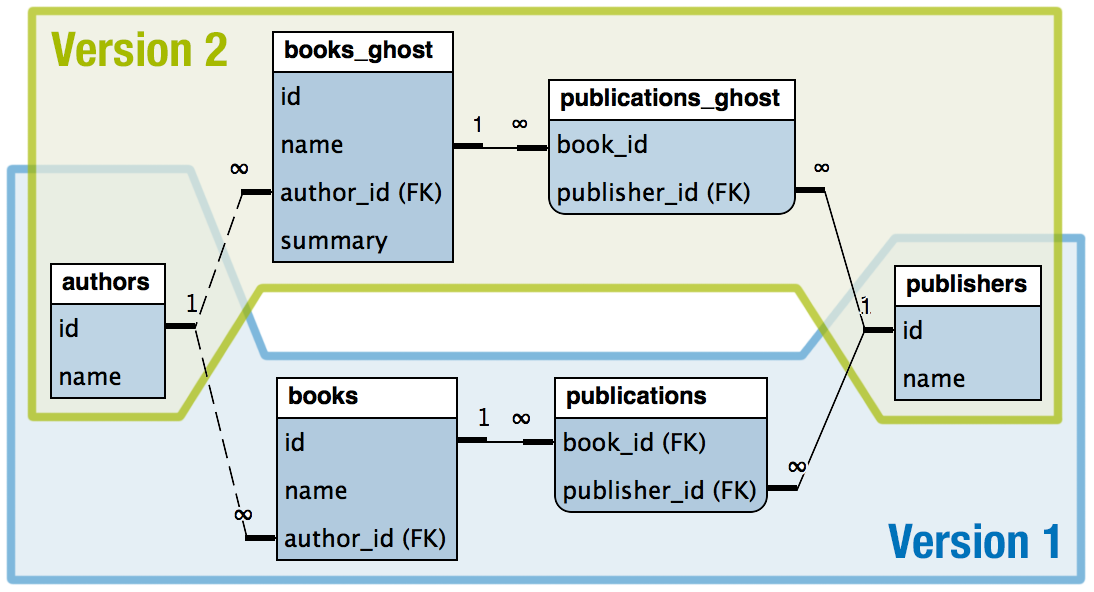
\includegraphics[width=3.0in]{in-migration-state.png} }}%
    \qquad
    \subfloat[New database schema, after migration]{{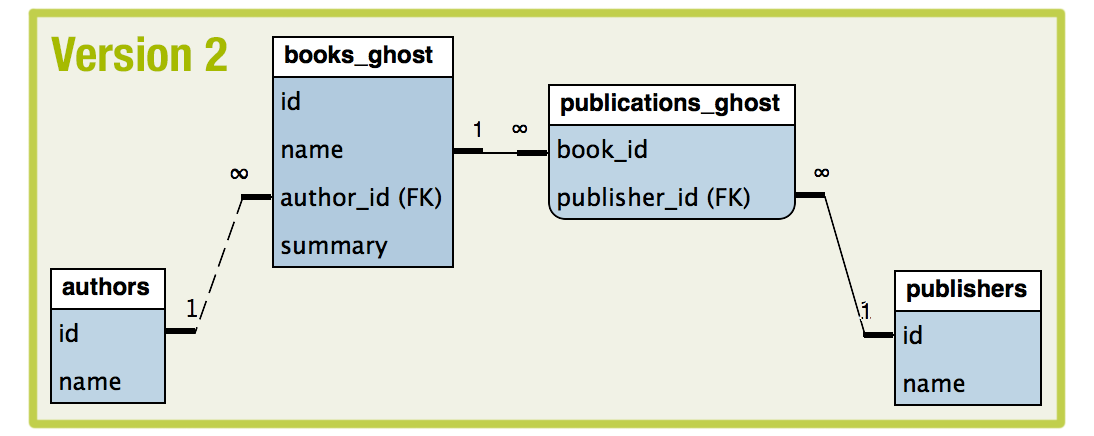
\includegraphics[width=3.0in]{post-migration-state.png} }}%
    \caption{Different stages of database schema during migration}%
    \label{fig:migration-stages}%
\end{figure}

QuantumDB currently consists of two parts: 
\begin{itemize}
  \item{\textbf{qdb:core} is the program responsible for performing the actual migration tasks on the database. It does this by creating ghost tables of tables under change, using triggers to keep the ghost tables and the original tables synchronized with each other, and a background task which copies the data from the original tables to the ghost tables in small batches to prevent degrading the performance of the database.}
  \item{\textbf{qdb:driver} is a Java JDBC driver which can wrap another JDBC driver. When used, the software engineers can specify a database schema version on which that version of their application operates. The driver then rewrites SQL queries sent to it by the application, and passes them on to the wrapped database JDBC driver which in turn sends them to the database. When rewriting queries, it replaces table names with the names of the associated (ghost) table names where applicable.}
\end{itemize}

With QuantumDB we can currently take one of the active database schemas, apply an arbitrary number of schema operations to it, and expose the resulting database schema in addition to the original database schema. Once the last application connected to a particular version of the database schema disconnects, the tables associated with that database schema version can be safely discarded.

\section{Initial Measurements} %(0.5)

In order to validate our work at an early stage we have setup a small experiment to verify that the proposed approach and our implementation of it behaves as expected. 

\subsection{Setup}
We have installed PostgreSQL 9.3 and a small test application --- made available on GitHub~\cite{QuantumDB-RelEng-Demo} --- on a server with a 4-core Intel Core i7-3770, a 1TB hard disk, and 16GB memory. The test application inserts 50 million records into a single table called ``users'' and starts a simple demo application with two threads which continuously query and manipulate the data in that table using SELECT, INSERT, UPDATE, and DELETE statements. It then uses one of two methods to add a non-nullable column to the ``users'' table. During this process we keep track of the duration of the queries issued by the demo application and how long each method takes to complete. 

The ``naive'' approach simply executes an ``ALTER TABLE users ADD COLUMN'' statement to add the new column to the database. Once this statement has completed, we can start a new demo application which can operate on the new structure of the ``users'' table. Since the new structure of the ``users'' table is compatible with both the old and the new version of the demo application they can run in parallel to each other, allowing for any kind of deployment method to be used. 

The second approach uses QuantumDB to add the new column. It first creates a ghost table based on the ``users'' table with the new column. It then iteratively copies records from the ``users'' table to the ghost table in batches of 2,000 records at intervals of 50 milliseconds. With this we attempt to avoid negatively affecting the performance of the queries issued by the demo application while we are copying the records. Unlike with the previous approach, with this approach the demo applications use the QuantumDB JDBC driver which exposes each demo application to a different version of the database schema (containing either the ``users'' table or the ghost table). The driver ensures that each query is rewritten in such a way that the correct table is queried for that specific version of the schema.


\subsection{Results}
\label{sec:results}

The total migration time for the ``naive'' approach was 2 minutes and 26 seconds, during which the demo application was unable to read from or write to the database. The total migration time for the QuantumDB approach was 50 minutes and 41 seconds. Although significantly slower than the ``naive'' approach, the demo applications remained operational throughout this period (see Figure~\ref{fig:migration}).

\begin{figure}%
    \centering
    \subfloat[Before migration]{{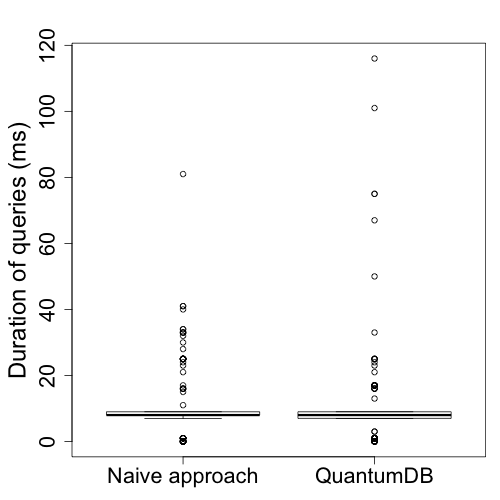
\includegraphics[width=1.55in]{normal-operations.png} }}%
    \qquad
    \subfloat[During migration]{{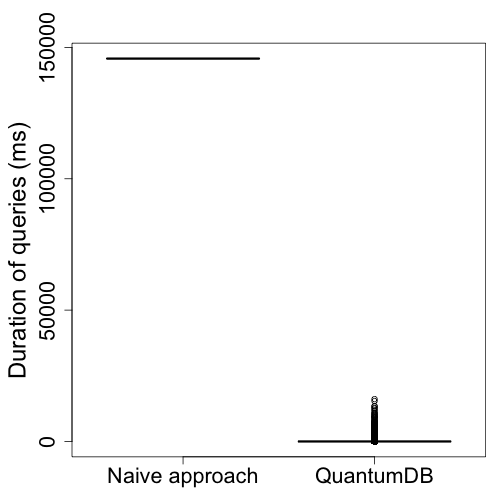
\includegraphics[width=1.55in]{migration.png} }}%
    \caption{Query performance of demo application before and during migration}%
    \label{fig:migration}%
\end{figure}

It is worth noting that we have not invested any time in improving the performance of QuantumDB or reducing the performance impact it has on the database and its clients. During this experiment we noticed that the hard disk was periodically unable to write data to disk quickly enough. As a result queries were taking significantly longer than normal to complete. We are confident that we can greatly reduce this by tweaking the PostgreSQL config, switching to a faster hard disk, or lowering the rate of migration during the copy phase.

\section{Road ahead}
As stated before, work on QuantumDB is not finished. To be able to use QuantumDB effectively in production environments we still need to work on the following issues: 

\begin{itemize}
  \item{QuantumDB can already deal with foreign keys referring from tables under change to other tables not under change. To fully support foreign keys QuantumDB would also need to be able to handle foreign keys referring to tables under change. This is currently being worked on.}
  \item{Use performance metrics to throttle the copy phase. When the database is (too) busy (high disk I/O, high CPU usage, or memory starvation), we should slow down the iterative copy process. Vice-versa we can speed it up when the database is not under load.}
  \item{QuantumDB currently only supports PostgreSQL, but since most SQL databases have support for triggers and procedures of some kind, this should prove easily extendable to other popular SQL databases.}
  \item{The driver currently uses a very rudimentary query rewriting algorithm to replace table names under change with the names of ghost tables. It does not yet support the entire PostgreSQL query syntax.}
\end{itemize}



% An example of a floating figure using the graphicx package.
% Note that \label must occur AFTER (or within) \caption.
% For figures, \caption should occur after the \includegraphics.
% Note that IEEEtran v1.7 and later has special internal code that
% is designed to preserve the operation of \label within \caption
% even when the captionsoff option is in effect. However, because
% of issues like this, it may be the safest practice to put all your
% \label just after \caption rather than within \caption{}.
%
% Reminder: the "draftcls" or "draftclsnofoot", not "draft", class
% option should be used if it is desired that the figures are to be
% displayed while in draft mode.
%
%\begin{figure}[!t]
%\centering
%\includegraphics[width=2.5in]{myfigure}
% where an .eps filename suffix will be assumed under latex,
% and a .pdf suffix will be assumed for pdflatex; or what has been declared
% via \DeclareGraphicsExtensions.
%\caption{Simulation Results}
%\label{fig_sim}
%\end{figure}

% Note that IEEE typically puts floats only at the top, even when this
% results in a large percentage of a column being occupied by floats.


% An example of a double column floating figure using two subfigures.
% (The subfig.sty package must be loaded for this to work.)
% The subfigure \label commands are set within each subfloat command, the
% \label for the overall figure must come after \caption.
% \hfil must be used as a separator to get equal spacing.
% The subfigure.sty package works much the same way, except \subfigure is
% used instead of \subfloat.
%
%\begin{figure*}[!t]
%\centerline{\subfloat[Case I]\includegraphics[width=2.5in]{subfigcase1}%
%\label{fig_first_case}}
%\hfil
%\subfloat[Case II]{\includegraphics[width=2.5in]{subfigcase2}%
%\label{fig_second_case}}}
%\caption{Simulation results}
%\label{fig_sim}
%\end{figure*}
%
% Note that often IEEE papers with subfigures do not employ subfigure
% captions (using the optional argument to \subfloat), but instead will
% reference/describe all of them (a), (b), etc., within the main caption.


% An example of a floating table. Note that, for IEEE style tables, the
% \caption command should come BEFORE the table. Table text will default to
% \footnotesize as IEEE normally uses this smaller font for tables.
% The \label must come after \caption as always.
%
%\begin{table}[!t]
%% increase table row spacing, adjust to taste
%\renewcommand{\arraystretch}{1.3}
% if using array.sty, it might be a good idea to tweak the value of
% \extrarowheight as needed to properly center the text within the cells
%\caption{An Example of a Table}
%\label{table_example}
%\centering
%% Some packages, such as MDW tools, offer better commands for making tables
%% than the plain LaTeX2e tabular which is used here.
%\begin{tabular}{|c||c|}
%\hline
%One & Two\\
%\hline
%Three & Four\\
%\hline
%\end{tabular}
%\end{table}


% Note that IEEE does not put floats in the very first column - or typically
% anywhere on the first page for that matter. Also, in-text middle ("here")
% positioning is not used. Most IEEE journals/conferences use top floats
% exclusively. Note that, LaTeX2e, unlike IEEE journals/conferences, places
% footnotes above bottom floats. This can be corrected via the \fnbelowfloat
% command of the stfloats package.



\section{Conclusion} 

Although development of QuantumDB is still ongoing, initial measurements are promising. With our small test application we have shown that we can migrate from one database schema to a state where both the old and the new database schemas are active, while still enabling database clients to remain operational. Applications can connect with the database according to a specific schema version, and no longer have to deal with database schemas being in an in-between state. This should effectively allow further decoupling of the release process from the development process. We believe that this approach can put \textit{Continuous Deployment} and \textit{Canary Releases} in reach of more software and release engineers.




% conference papers do not normally have an appendix


% use section* for acknowledgement
%\section*{Acknowledgment}


%The authors would like to thank...





% trigger a \newpage just before the given reference
% number - used to balance the columns on the last page
% adjust value as needed - may need to be readjusted if
% the document is modified later
%\IEEEtriggeratref{8}
% The "triggered" command can be changed if desired:
%\IEEEtriggercmd{\enlargethispage{-5in}}

% references section

% can use a bibliography generated by BibTeX as a .bbl file
% BibTeX documentation can be easily obtained at:
% http://www.ctan.org/tex-archive/biblio/bibtex/contrib/doc/
% The IEEEtran BibTeX style support page is at:
% http://www.michaelshell.org/tex/ieeetran/bibtex/
%\bibliographystyle{IEEEtran}
% argument is your BibTeX string definitions and bibliography database(s)
%\bibliography{IEEEabrv,../bib/paper}
%
% <OR> manually copy in the resultant .bbl file
% set second argument of \begin to the number of references
% (used to reserve space for the reference number labels box)

\bibliographystyle{plain}
\bibliography{paper}

% \begin{thebibliography}{1}
% 
% \bibitem{IEEEhowto:kopka}
% H.~Kopka and P.~W. Daly, \emph{A Guide to \LaTeX}, 3rd~ed.\hskip 1em plus
%   0.5em minus 0.4em\relax Harlow, England: Addison-Wesley, 1999.
% 
% \end{thebibliography}




% that's all folks
\end{document}


